\chapter{Introduction}

Rutherford discovered in 1911 that the atomic nuclei are composed of a dense nucleus surrounded by an electron cloud, and eventually that the nucleus if composed of positive and neutral spin 1/2 particles called protons and neutrons. The proton and neutron are actually composed of 3 fundamental particles called quarks. Besides for the charge differences between protons and neutrons, they exhibit a fundamental symmetry which explains their almost identical mass. Typically neutrons and protons are treated as two different isospin projections of a ``nucleon", (-1/2 and 1/2) respectively.



The nucleus itself accounts for 99.9\% of the mass of the atom and only \num{e-12} of the total volume, making it incredibly dense. Without a balancing force the Coulomb force between protons would render the nucleus unstable. The nuclear strong interaction is the fundamental force governing the interactions between the constituent quarks in the nucleons, deriving its name from the large force which acts only over small distances. The strong force is attractive only for a small regions approximately \SIrange{1}{2}{\femto\metre} and becomes very repulsive at even shorter distances. It is for this reason that the distance between nuclei is a near constant value, and therefore the density is remarkably constant over a wide range of nuclei CITE HERE. This density is referred to as the  \emph{saturation density}, $\rho_0 = \SI{1.7e14}{\gram\per\centi\metre\cubed}$.  

 In this way nuclei can be thought of as an in-compressible liquid. This picture was remarkably successful at describing the binding energies of nuclei at saturation density. The Bethe-Weizsacker semi-empirical formula predicts the binding energy as a function of the number of neutrons $N$, protons $Z$, and total nucleons $A = Z + N$, where the binding energy per nucleon is $\epsilon/A$:
 
\begin{equation}
\frac{\epsilon}{A} = a_vA - a_s A^{2/3} - a_c \frac{Z^2}{A^{1/3}} - a_A\frac{(N - Z)^2}{A} + \mathcal{O}
\label{eq:semiEmp}
\end{equation}

Since the number of nucleons is related to the volume of the nucleus, the volume term ,$a_V$, originates from the the saturation of the strong force and its short range nature. There are correction terms accounting for the surface, $a_s$, since nucleons near the surface do not have as many neighbors as nucleons inside, and the coulomb term which is related to the size of the nucleus which scales as $A^{1/3}$. The asymmetry term, $a_A$, is related to the cost in energy one pays to become more neutron or proton rich; it is typically referred to as the \emph{Symmetry Energy}. This originates from pauli blocking where it is more energetically favorable to form neutron-proton pairs since their isospin numbers are different. The di-neutron and di-proton form part of the isospin triplet only allowing for the total isospin $T=1$, where as the deuteron (neutron-proton) system may form $T={0,1}$ in the singlet or the triplet, with the singlet being more energetically favorable. 

Large macroscopic objects such as neutron stars are composed of mostly pure neutron matter CITE HERE, which is normally not stable. The large extent of the star allows for the gravitational force to balance the strong force creating a compact dense star. The pressures vary in the neutron star from low densities near the crust to the dense interior which can reach up to 9$\rho_o$ CITE HERE. To understand these exotic systems, the energy density of the system must be described in a more general way than Eq.~\ref{eq:semiEmp} to describe matter over a wide range of densities. 

Guided by Eq.~\ref{eq:semiEmp}, we can separate the energy density $E$ of a system into two components,

\begin{equation}
E(\rho,\delta) = E(\rho	) + S(\rho)\delta^2,
\label{eq:energyEos}
\end{equation}

where $E(\rho)$ describes the symmetric term (i.e. independent of isospin), and the symmetry energy $S(\rho)$ which depends on the asymmetry of the system, written now in terms of the neutron and proton densities, 

\begin{equation}
\delta = \frac{\rho_n - \rho_p}{\rho}.
\label{eq:asym}
\end{equation}

The Equation of State (EoS) of nuclear matter can be calculated by, 

\begin{equation}
P = \Big(\frac{\delta E}{\delta V}\Big)\vert_{T=0,N} = -\rho^2 \frac{\delta E}{\delta \rho}\Big)\vert_{T=0,N}, 
\label{eq:pressEos}
\end{equation}

for a fixed number of particles $N$ and zero temperature. One can extend to higher temperatures by adding the Boltzman dependence CITE HERE. The partial derivative with respects to volume can be rewritten in terms of density:

\begin{equation}
P = -\rho^2 \frac{\delta E}{\delta \rho}\vert_{T=0,N}.
\label{eq:densEos}
\end{equation}

To understand macroscopic pressures in the neutron star, which balance the gravitational force, we must understand the density dependence of the symmetry energy. 

\section{Density Dependence of the Symmetry Energy}
In the last couple decades, the symmetric term of Eq.~\ref{eq:energyEos} has been determined for a wide range of densities ranging from $\rho_0 - 9\rho_0$ CITE HERE. In contrast, the symmetry energy has only been experimentally constrained for densities at or below $\rho_0$. Figure~\ref{fig:symDen} shows some of the experimental constraints which have been performed by a series of independent measurements and observables CITE HERE ALL. Typically an effective interaction is used to describe the phenomenological observations of nucleon-nucleon interactions observed in nuclei. One of such interactions is described by the Skyrme interaction, which typically is described by a multi-parameter function which takes into account momentum dependence (through an effective mass), 2-body interactions, and correlations CITE HERE. Several Skyrme parameterizations are shown as lines in Fig.~\ref{fig:symDen}. Though most of the functional forms satisfy the experimental constraints at low densities there is a considerable uncertainty at high densities, which are more relevant to neutron stars. 




\section{Heavy Ion Collisions}
Besides observing neutron stars directly, heavy-ion collisions (HIC) provide the only way we can probe the density dependence of the symmetry energy in the laboratory setting. When two nuclei collide in a collision, in the very early stages they compress to form a high density region where the nuclei overlap. This momentary density can reach up to $3\rho_0$ depending on the incident beam energy. HICs provide the only way we can probe the isospin asymmetry dependence of the nuclear EoS. This is accomplished by using radioactive neutron-rich beams to collide on stable targets. 

The pressure arising from the symmetry energy depends on the curvature of the symmetry energy at a given density. If the density dependence of the symmetry energy is positive at high densities the symmetry energy would work to force neutrons out of the system. Where as if the derivative was negative the symmetry energy would attract neutrons. It is this pressure that is driving the dynamics of neutrons and protons. By measuring protons and neutrons we can see signatures of the effects of the symmetry energy in the final spectra of these particles. Measuring neutrons experimentally can be quite challenging and space is limited by large neutron wall arrays CITE HERE. Also, though the overlap region temporarily reaches a high density, the neutrons which participated in this region also evolve through regions of lower densities until they reach their final state, diluting the signal from the dense region. 


\begin{figure}
\centering

\includegraphics[scale=.01]{place}
\caption{Experimental constraints of the density dependence of the symmetry energy}
\label{fig:symDen}
\end{figure}


\section{Pion Observable}
It is preferable to find an observable that is easier to measure experimentally than neutrons, and is more sensitive to the high density region. Pions are produced though and intermediate process where nucleon-nucleon collisions form an excited $\Delta$ baryon resonance from one of the nucleons, which then decay decay shortly after into a pion:

\begin{equation}
\ce{ NN <=> \Delta N <=> \pi NN}.
\end{equation}


It has been shown in \cite{mingzhang} that most of the $\Delta$'s are produced in the early dense regions of the collision. Figure~\ref{fig:deltaProduction} shows the average local density (c) which $\Delta$'s are produced and the number in the system (b), as a function of time in the simulation of Au + Au collisions at \SI{400}{\MeVA}. Panel (a) shows the density distribution of the density at the moment of creation for $\Delta$'s. Since the average lifetime of the $\Delta$  is $\tau_{\Delta} = \SI{1.7}{\femto\metre\per\clight}$, the $\Delta$ resonance has very little time to be affected by the medium before decaying into a $\pi$ and nucleon. Thus the outgoing $\pi$ is contains information on the high density region of the collision. 

\begin{figure}[!htb]
\centering
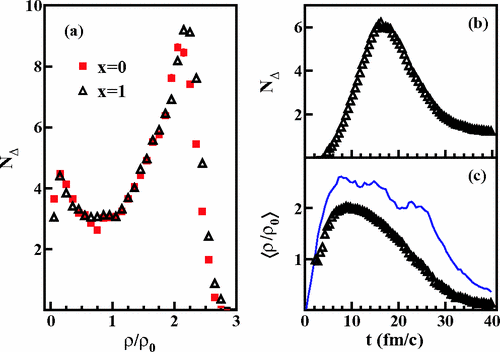
\includegraphics[scale=.2]{deltaProduction.png}
\caption{Figure taken from \cite{mingzhang} for Au + Au collisions at \SI{400}{\MeVA}. Panel (a) shows the density in the region of the $\Delta$ resonance creation for two different symmetry energies (x=0 soft) and (x=1 stiff). Panel (b) and (c) show the evolution of collision in time steps, where (b) shows the number of deltas in the system as a function of time and (c) shows the mean local baryon density in the region where $\Delta$ resonances are produced. The blue line in (c) represents the average baryon density in the most central region of the collision. This evidence shows that a majority of $\Delta$'s are produced in the high density region of the early collision.}
\label{fig:deltaProduction}
\end{figure}

The branching ratio of the various flavors of $\Delta$'s is given by the Clebsh-Gordon coefficients as shown in \ref{appen:deltadecay}. Here we see that in general proton-proton collisions give rise primarily to  $\pi^+$ and neutron-neutron collisions give rise to primarily $\pi^-$. In this $\Delta$ resonance model the charged pion ratio can be described as,

\begin{equation}
\frac{\pi^-}{\pi^+} = \frac{ 5pp + pn }{5nn + pn}.
\label{eq:deltaModel}
\end{equation}

In this $\Delta$ resonance model, $\pi^-/\pi^+ \approx (N/Z)^2$ where $N/Z$ is the neutron-proton ratio of the dense central collision where they are produced. Pions can be reabsorbed into a $\Delta$ resonance after colliding with the another nucleon in the froward and backwards process $\ce{\Delta <=> \pi N}$. This process generally dilutes the pion sensitivity to the high density region, since with each absorption and re-emission would change the pion dynamics or even the charge of the pion which would reflect the asymmetry at the point of creation and eventual re-emission. Total pion absorption back into two nucleons requires a three body process where a pion is absorbed creating a $\Delta$ resonance, then another nucleon must collide with the resonance to create two nucleons. Because of this, the total pion absorption (removing pions totally) is a less frequent effect than the absorption re-emission process. Yet in general by measuring the $\pi^-$ and $\pi^+$ is connected with n-n and p-p collisions. Instead of measuring neutrons we can measure the $\pi^-$ which is much easier to measure experimentally. 

%nuclear chart
%Dense nuclear matter 
%Liquid drop model explain density around saturation
%explain symmetry energy 
%extend to systems of larger pressure, isospin assymetry 
%symmetry energy how to calculate 
%Previous constraints on symmetry energy
%heavy ion collisions only way to probe density and 
%dynamics of proton neutrons 

%pion production 




















\section{From Nuclear Forces to the Equation of State}
Isospin as a good quantum number at low energies 
Figure showing the nuclear forces for the pp, pn, nn 
Pauli exclusion 
inter particle distance , saturation density (maybe figure of all densities?)
Building the infinite matter
Statistical model 
Forces manifest in Energy/particle 

\section{The Nuclear Equation of State}
Figure showing the binding energy vs p-n asym
Liquid drop model, mass equation, move to higher densities
Symmetric EoS asymmetric EoS(symmetry energy)
Density dependence of the symmetry energy 

\section{Phases of Nuclear Matter}
gas liquid phase, gas, where are we
Progression through the heavy ion collision 
liquid, liquid gas, gas 

\section{Studying EoS through Heavy Ion Collisions}
going from infinite matter to finite matter 
approximate nuclear matter with neutron rich radioactive ion beams
probe different asymmetries 
probe different densities with different beam energies 
Symmetry energy goes down at higher beam energies

\section{Boltzmann Ulong Uhlenbeck (BUU) Transport Code}
Does not reach equilibrium for all observable (hadrons) what about pions?
Build up a mean field picture (momentum dependent) unknown quantities here
Non equilibrium can be solved with Boltzman equation with collision term and solved by MC
Figure of transport simulation code showing collision progression 
Clustering is an issue 
Meson, resonance production 

\section{Observables of interest to the EoS}
Particle yields of isospin opposites 
Flow??
Figure showing p-n observable lessens at high energy and from all densities 

\section{Pion Production }
Figure showing delta resonance 
Figure showing pion's produced at 2po 
Figure showing fermi motion effect (not really sub threshold but ok)
(chemical potential model, delta isobar) prediction for pion ratio
pion mass is small momentum shifted by coulomb affecting shape of pion spectra

\section{Previous Constraints}
Figure showing GW constraint and other previous constraints 
FOPI data at 400 A MeV not as sensitive to symmetry energy 
Saturation density and lower constrained but issues at high density
conflicting analysis on FOPI data which was not intended to be used for Symm Energy
Can you group all the constraints to one nice plot???

\section{Motivation for building the S$\pi$RIT TPC}
Based on EOS TPC
High efficiency for detecting pions and other light charged particles 
Effort to reduce the experimental error bars on such spectra which theory could use


